
\documentclass[a4paper,12pt]{article}

\usepackage{graphicx} % Required for inserting images
\usepackage{amsmath,amssymb,amsfonts}
\usepackage{subcaption}
% -----------------------
% Package Imports
% -----------------------

% Set page margins
\usepackage[a4paper, top=1in, bottom=0.8in, left=1.1in, right=0.8in]{geometry}

% Use Times New Roman font
\usepackage{times}

% Add page numbering
\pagestyle{plain}

% Enable graphics inclusion
\usepackage{graphicx}
\usepackage{float}
% Enable code listings
\usepackage{listings}
\usepackage{xcolor} % For customizing code colors
\setlength{\parindent}{0pt}




\begin{document}
	\section{Experiment No. 1}
	
	\section{Experiment Title }
	
    Introduction to different DC and AC Machines and General discussion on safety and precautions

	\section{Objective}
	
	The objectives of this lab are as follows:
	\begin{itemize}
		\item To investigate the torque and speed characteristics of a DC motor.
		\item To understand the relationship between torque and speed for DC motors.
		\item To observe the effect of varying load on the motor's speed and torque.
	\end{itemize}
	
	\section{Theory}
	A machine is a device that uses energy to perform a specific task. It can be mechanical, electrical, or a combination of both. Machines typically convert one form of energy into another to accomplish work.
	power supply
	three phase asynchronous motor
	three phase synchronous
	tachogenerator
	AC-DC Multimeter
	Dc Current Stator
	Universal Motor
	Resistors
	230V. DC Supply
	3 point starter
	
	\section{Types of DC and AC Machines}
	
	\subsection{DC Machines}
	DC machines are commonly used in applications requiring variable speed control and high starting torque. They are classified into:
	\begin{itemize}
		\item \textbf{DC Motors}: Convert electrical energy into mechanical energy.
		\item \textbf{DC Generators}: Convert mechanical energy into electrical energy.
	\end{itemize}
	Based on excitation, DC machines are further classified as:
	\begin{itemize}
		\item Separately excited DC machines
		\item Shunt-wound DC machines
		\item Series-wound DC machines
		\item Compound-wound DC machines
	\end{itemize}
	
	\subsection{AC Machines}
	AC machines are widely used due to their efficiency and robustness. They are classified into:
	\begin{itemize}
		\item \textbf{Induction Machines}: Work on the principle of electromagnetic induction.
		\item \textbf{Synchronous Machines}: Operate at a constant speed determined by the supply frequency.
		\item \textbf{Transformers}: Used to step up or step down voltage levels.
	\end{itemize}
	
	\section{Description of Machines}
	
	\subsection{Three-Phase Asynchronous Motor}
	A three-phase asynchronous motor, also known as an induction motor, operates on the principle of electromagnetic induction. It is widely used in industrial applications due to its robustness and self-starting capability.
		\begin{figure}[H]
		\centering
		\includegraphics[width=0.7\linewidth]{"Images/1"}
		\caption{LCD/LED TV Trainer}
		
	\end{figure}
	\subsection{Three-Phase Synchronous Motor}
	A three-phase synchronous motor runs at a constant speed determined by the supply frequency. It requires external excitation and is commonly used in applications requiring precise speed control.
	
	\subsection{Tachogenerator}
	A tachogenerator is a device used to measure the rotational speed of a shaft. It converts mechanical motion into a proportional electrical signal.
	
	\subsection{AC-DC Multimeter}
	An AC-DC multimeter is an instrument used to measure voltage, current, and resistance in both AC and DC circuits.
	
	\subsection{DC Current Stator}
	A DC current stator is a stationary part of a DC machine that produces a magnetic field necessary for the operation of the motor or generator.
	
	\subsection{Universal Motor}
	A universal motor is a type of electric motor that can operate on both AC and DC power supplies. It is commonly found in household appliances like mixers and drills.
	
	\subsection{Resistors}
	Resistors are passive electrical components that limit the flow of current in a circuit, helping in voltage regulation and circuit protection.
	
	\subsection{230V DC Supply}
	A 230V DC supply provides a stable direct current voltage for operating electrical machines and circuits requiring high voltage DC power.
	
	\subsection{3-Point Starter}
	A 3-point starter is a protective device used to limit the inrush current when starting a DC motor, ensuring safe and efficient operation.
	
	\section{Safety and Precautions}
	Handling electrical machines requires adherence to safety guidelines to prevent electrical hazards, injuries, and equipment damage. Some key precautions include:
	\begin{itemize}
		\item Always wear insulating gloves and shoes while working with electrical machines.
		\item Ensure proper grounding and insulation to avoid electrical shocks.
		\item Avoid touching live wires and rotating parts while machines are operational.
		\item Regularly inspect machines for loose connections and overheating.
		\item Follow manufacturer guidelines and safety procedures during operation and maintenance.
	\end{itemize}
	
	\section{Conclusion}
	DC and AC machines form the backbone of modern electrical applications, providing efficient energy conversion. Understanding their working principles and adhering to proper safety precautions ensures optimal performance and minimizes risks associated with their operation. This lab provided practical exposure to different types of electrical machines and their safety protocols, enhancing theoretical knowledge and practical skills.
	
		% DC Machine Specifications
	\subsubsection{DC Motor Specifications}
	\begin{table}[H]
		\centering
		\caption{DC Motor Specifications}
		\begin{tabular}{| c | c |}
			\hline
			\textbf{Specification} & \textbf{Value} \\ \hline
			Power Rating & 300 W\\ \hline
			Voltage Rating [EXC.SERIES \& EXC. SEP] & 220 V \\ \hline
			Current Rating [EXC SERIES] & 1.9 A \\ \hline
			Current Rating [EXC SEP] & 1.8 A \\ \hline
			Vexc & 220 V \\ \hline
			Iexc & 0.1 A \\ \hline
			Speed & 2500 RPM \\ \hline
			
		\end{tabular}
		
		
		\label{tab:2}
	\end{table}
	
		% DC Generator Specifications
	\subsubsection{DC Generator Specifications}
	\begin{table}[H]
		\centering
		\caption{DC Generator}
		\begin{tabular}{| c | c |}
			\hline
			\textbf{Specification} & \textbf{Value} \\ \hline
			Power Rating & 300 W\\ \hline
			Voltage Rating [EXC.SERIES] & 210 V \\ \hline
			Voltage Rating [ EXC. COMP] & 220 V \\ \hline
			Current Rating [EXC SERIES \& EXC COMP] & 1.4 A \\ \hline
			Vexc & 0-220 V \\ \hline
			Iexc & 0.11 A \\ \hline
			Speed & 3000 RPM \\ \hline
			
		\end{tabular}
		
		\label{tab:2}
	\end{table}
	
	\subsubsection{Single-Phase Transformer Specifications}
	\begin{table}[H]
		\centering
		\caption{Single-Phase Transformer Specifications}
		\begin{tabular}{| c |c |}
			\hline
			\textbf{Specification} & \textbf{Value} \\ \hline
			Power Rating & 760 kVA \\ \hline
			$U_1$  & 230 V \\ \hline
			$U_2$  & 400V-230V \\ \hline
			$I_1$ & 3.7 A \\ \hline
			$I_2$ & 1A-1.7A \\ \hline
			Frequency & 50 Hz \\ \hline
			
		\end{tabular}
		
		
		\label{tab:3}
	\end{table}
	
	
	
	\section{Required Apparatus}
	\begin{enumerate}
		\item Electric Machine Trainer
		\begin{enumerate}
			\item DC Motor Starting Resistor
			\item DC Power Supply (Rating: Voltage: 200V)
			\item DC Ammeters (Rating: Current: 5A)
			\item DC Voltmeter (Rating: Voltage: 500V)
			\item DC Motor Field Resistor
			\item Speed Meter (Rating: 1500 rpm max)
			\item Torque Meter (Rating: 0.24 kg-m max)
		\end{enumerate}
		
		
		\item DC Compound Motor (Ratings: Output: 360W, Voltage: 200V, Current: 2.5A, Speed: 1500 rpm;  Field: 0.2A, Pole: 2P)
		\item Dynamometer (Ratings: Output: 360W, Voltage: 100V, Current: 3A; Pole: 2P; Speed: 4000 rpm max, Type: Eddy Current)
		
	\end{enumerate}
	\newpage
	\section{Circuit Diagrram}
	
	
	
	
	
	\newpage
	
	
	
	
	
	
	\section{Graph}
	
	
	
	
	
	\begin{figure}[H]
		\centering
		\begin{subfigure}[t]{1\textwidth}
			\centering
			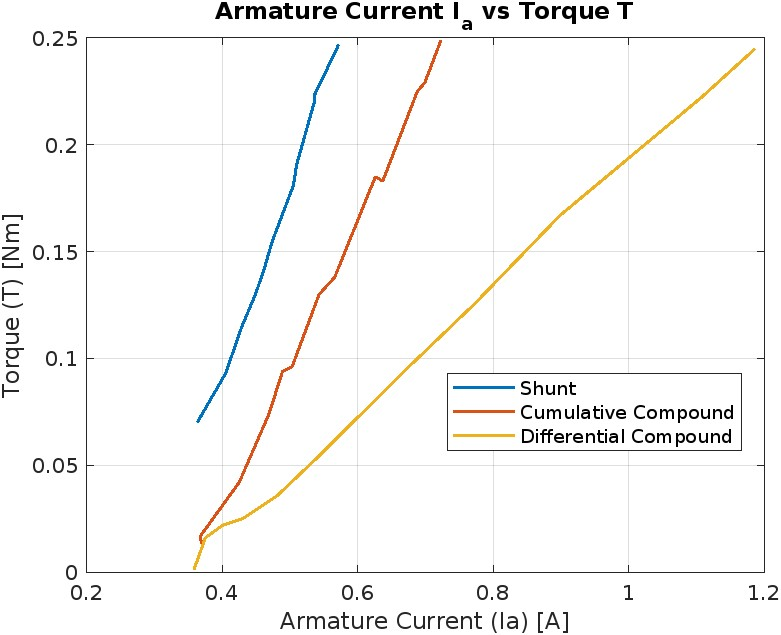
\includegraphics[width=0.85\linewidth]{Images/1.2}
			\caption{ $I_a$ vs. Torque (T) Graph }
			\vspace{0.1cm}
		\end{subfigure}
		
		\begin{subfigure}[t]{1\textwidth}
			\centering
			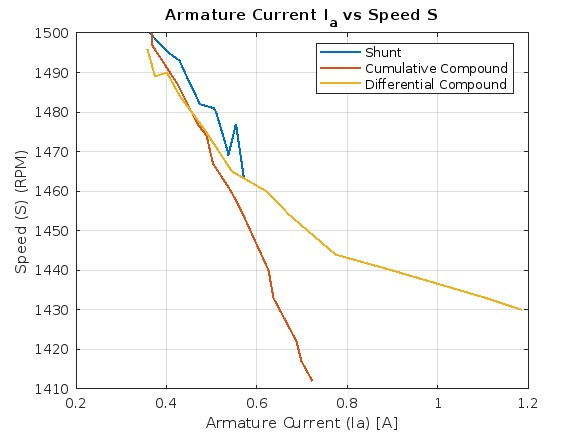
\includegraphics[width=0.95\linewidth]{Images/2.1}
			\caption{ $I_a$ vs. Speed(S) Graph}
		\end{subfigure}
		
		
	\end{figure}
	
	\section{Discussion}
	
	The experiment was conducted to investigate the Torque and Speed Characteristics of a DC Motor. The relationship between torque and speed can be described by the following equations:
	
	\begin{equation}
		T = K I_a \Phi
	\end{equation}
	
	\[
	S = \frac{V_T - I_a R_a}{K \Phi}
	\]
	
	To start the motor, it was carefully ensured that the starting resistance was kept at its maximum value, and the field resistance was also kept at its maximum. Then, the voltage of the supply was increased to 100V. After that, the starting resistance was decreased. The supply voltage was further increased to 200V, and the field resistance was then decreased to speed up the motor to 1500 rpm, the rated speed of the motor.
	
	There were three knobs to adjust the torque value of the electrodynamometer. Initially, the torque was set to zero by adjusting the knob. Data was then recorded for the armature current, torque value, and speed at different torque levels for the DC shunt and compound motors.
	\section{Introduction}
	Electric machines play a crucial role in modern electrical engineering, converting electrical energy into mechanical energy and vice versa. These machines are broadly classified into DC (Direct Current) machines and AC (Alternating Current) machines. This report discusses various types of DC and AC machines, their working principles, and their applications. Additionally, safety measures and precautions associated with handling these machines are discussed to ensure proper operation and accident prevention.
	
	\section{Types of DC and AC Machines}
	
	\subsection{DC Machines}
	DC machines are commonly used in applications requiring variable speed control and high starting torque. They are classified into:
	\begin{itemize}
		\item \textbf{DC Motors}: Convert electrical energy into mechanical energy.
		\item \textbf{DC Generators}: Convert mechanical energy into electrical energy.
	\end{itemize}
	Based on excitation, DC machines are further classified as:
	\begin{itemize}
		\item Separately excited DC machines
		\item Shunt-wound DC machines
		\item Series-wound DC machines
		\item Compound-wound DC machines
	\end{itemize}
	
	\subsection{AC Machines}
	AC machines are widely used due to their efficiency and robustness. They are classified into:
	\begin{itemize}
		\item \textbf{Induction Machines}: Work on the principle of electromagnetic induction.
		\item \textbf{Synchronous Machines}: Operate at a constant speed determined by the supply frequency.
		\item \textbf{Transformers}: Used to step up or step down voltage levels.
	\end{itemize}
	
	\section{Safety and Precautions}
	Handling electrical machines requires adherence to safety guidelines to prevent electrical hazards, injuries, and equipment damage. Some key precautions include:
	\begin{itemize}
		\item Always wear insulating gloves and shoes while working with electrical machines.
		\item Ensure proper grounding and insulation to avoid electrical shocks.
		\item Avoid touching live wires and rotating parts while machines are operational.
		\item Regularly inspect machines for loose connections and overheating.
		\item Follow manufacturer guidelines and safety procedures during operation and maintenance.
	\end{itemize}
	
	\section{Conclusion}
	DC and AC machines form the backbone of modern electrical applications, providing efficient energy conversion. Understanding their working principles and adhering to proper safety precautions ensures optimal performance and minimizes risks associated with their operation. This lab provided practical exposure to different types of electrical machines and their safety protocols, enhancing theoretical knowledge and practical skills.
	
	
\end{document}
